%----------------------------------------------------------------------------------------
% ct_grid.tex
%----------------------------------------------------------------------------------------

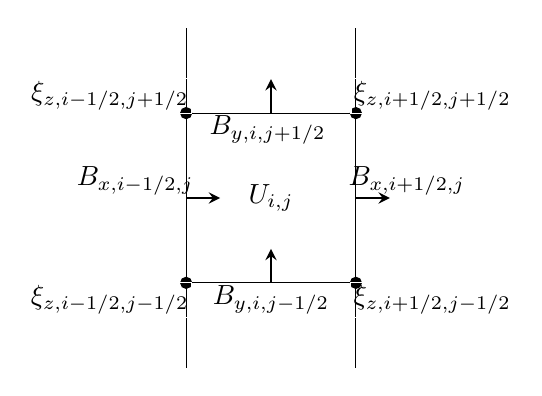
\begin{tikzpicture}[scale = {0.0125\linewidth},%inner sep = 1pt,
  >=stealth, %
  inner sep=1pt, outer sep=0pt,%
  axis/.style={thick,->},
  base node/.style={circle,draw,minimum size=4pt},
  wave/.style={thick,color=#1,smooth},
  polaroid/.style={fill=black!60!white, opacity=0.3}]

%% \draw[line width=1pt] (0.0,0.0)--(1.0,0.0);
%% \draw[line width=1pt] (0.0,0.0)--(0.0,1.0);
%% \draw[line width=1pt] (0.0,1.0)--(1.0,1.0);
%% \draw[line width=1pt] (1.0,0.0)--(1.0,1.0);

\draw[] (0.0,0.25)--(1.0,0.25);
\draw[] (0.0,0.75)--(1.0,0.75);
\draw[] (0.25,0.0)--(0.25,1.0);
\draw[] (0.75,0.0)--(0.75,1.0);

\node[draw=white] (Ucc) at (0.5,0.5) {$\mbf{U}_{i,j}$};

\draw[-stealth,thick] (0.75,0.5) -- (0.85,0.5); 
\node[] at (0.9,0.55) {$B_{x,i+1/2,j}$};

\draw[-stealth,thick] (0.25,0.5) -- (0.35,0.5); 
\node[] at (0.1,0.55) {$B_{x,i-1/2,j}$};

\draw[-stealth,thick] (0.5,0.75) -- (0.5,0.85); 
\node[] at (0.49,0.7) {$B_{y,i,j+1/2}$};

\draw[-stealth,thick] (0.5,0.25) -- (0.5,0.35); 
\node[] at (0.5,0.2) {$B_{y,i,j-1/2}$};

\node[base node,fill = black] at (0.25,0.25) {};
\node[base node,fill = black] at (0.25,0.75) {};
\node[base node,fill = black] at (0.75,0.25) {};
\node[base node,fill = black] at (0.75,0.75) {};

\node[draw=white] (ez1) at (0.025,0.2) {$\xi_{z,i-1/2,j-1/2}$};
\node[draw=white] (ez2) at (0.975,0.2) {$\xi_{z,i+1/2,j-1/2}$};
\node[draw=white] (ez3) at (0.025,0.8) {$\xi_{z,i-1/2,j+1/2}$};
\node[draw=white] (ez4) at (0.975,0.8) {$\xi_{z,i+1/2,j+1/2}$};

%% \draw[-line width=1pt] (0,0.7)--(0,0.75);  
%% \draw[line width=1pt] (-0,0)--(-0.75,0);
%% \node[draw=white] (sr) at (0.58457,0.33750) {$S_r$};
%% \node[draw=white] (ssr) at (0.33750,0.58457) {$S^*_r$};
%% \node[draw=white] (cd) at (0.058830,0.67243) {$S_m$};
%% \node[draw=white] (ssl) at (-0.33750,0.58457) {$S^*_l$};
%% \node[draw=white] (sl) at (-0.58457,0.33750) {$S_l$};

%% \node[draw=white] (ur) at (0.43467,0.11647) {$\mbf{U}_{r}$};
%% \node[draw=white] (usl) at (0.31820,0.31820) {$\mbf{U}^*_{r}$};
%% \node[draw=white] (usr) at (0.11647,0.43467) {$\mbf{U}^*_{2r}$};
%% \node[draw=white] (usr) at (-0.11647,0.43467) {$\mbf{U}^*_{2l}$};
%% \node[draw=white] (usl) at (-0.31820,0.31820) {$\mbf{U}^*_{l}$};
%% \node[draw=white] (ul) at (-0.43467,0.11647) {$\mbf{U}_{l}$};

%% \draw (0,0) -- (sr);  
%% \draw (0,0) -- (ssr);  
%% \draw (0,0) -- (cd);  
%% \draw (0,0) -- (ssl);  
%% \draw (0,0) -- (sl);  

\end{tikzpicture}
